%-----------------------------------------------
% Template para criação de resumos de projectos/dissertação
% jlopes AT fe.up.pt,   Fri Jul  3 11:08:59 2009
%-----------------------------------------------

\documentclass[9pt,a4paper]{extarticle}

%% English version: comment first, uncomment second
\usepackage[portuguese]{babel}  % Portuguese
%\usepackage[english]{babel}     % English
\usepackage{graphicx}           % images .png or .pdf w/ pdflatex OR .eps w/ latex
\usepackage{times}              % use Times type-1 fonts
\usepackage[utf8]{inputenc}     % 8 bits using UTF-8
\usepackage{url}                % URLs
\usepackage{multicol}           % twocolumn, etc
\usepackage{float}              % improve figures & tables floating
\usepackage[tableposition=top]{caption} % captions
%% English version: comment first (maybe)
\usepackage{indentfirst}        % portuguese standard for paragraphs
%\usepackage{parskip}

%% page layout
\usepackage[a4paper,margin=30mm,noheadfoot]{geometry}

%% space between columns
\columnsep 12mm

%% headers & footers
\pagestyle{empty}

%% figure & table caption
\captionsetup{figurename=Fig.,tablename=Tab.,labelsep=endash,font=bf,skip=.5\baselineskip}

%% heading
\makeatletter
\renewcommand*{\@seccntformat}[1]{%
  \csname the#1\endcsname.\quad
}
\makeatother

%% avoid widows and orphans
\clubpenalty=300
\widowpenalty=300

\begin{document}

\title{\vspace*{-8mm}\textbf{\textsc{Electronic Assessment for Software Development Certifications}}}
\author{\emph{Nelson Daniel Ribeiro Mendes}\\[2mm]
\small{Dissertação realizada sob a orientação do \emph{Prof.\ João Pascoal Faria}}\\
\small{na \emph{Strongstep - Innovation In Software Quality, Lda}}}
\date{}
\maketitle
%no page number 
\thispagestyle{empty}

\vspace*{-4mm}\noindent\rule{\textwidth}{0.4pt}\vspace*{4mm}

\begin{multicols}{2}

\section{Motivação}\label{sec:motiva}

Com o efeito da globalização, assistimos a uma mudança no paradigma dos mercados atuais, mudança essa que forçou as organizações a melhorar os seus processos de modo a manter a sua competitividade e deste modo garantir uma posição favorável no mercado. Para que tal aconteça, é necessário que comecem a simplificar e a perder menos tempo nos processos, pois só assim é possível à organização focar-se no que realmente interessa: a criação de valor.

As certificações são um reconhecimento formal de uma organização que fornecem orientação e ferramentas, no sentido de garantir que os produtos e serviços vão de encontro às necessidades e requisitos dos clientes e a sua qualidade é constantemente melhorada.

As certificações são um reconhecimento formal de uma organização que fornecem orientação e ferramentas, no sentido de garantir que os produtos e serviços vão de encontro às necessidades e requisitos dos clientes e a sua qualidade é constantemente melhorada. Apesar de serem úteis para a organização, as certificações exigem um esforço muito elevado e consomem muito tempo. Por exemplo, o método SCAMPI exige um esforço elevado, sendo por vezes muito doloroso e custoso monetariamente para a organização.


O método SCAMPI é o método standard de avaliação para a melhoria de processos, associado ao modelo CMMI que é um modelo para as organizações melhorarem os seus processos e é exigido por muitos contratos do governo dos EUA, especialmente no âmbito do desenvolvimento de software. SCRAIM é a ferramenta que vai fornecer meios para simplificar esse tipo de avaliações, com o objetivo de economizar tempo e consequentemente dinheiro.


\section{Objetivos}\label{sec:goals}

O suporte de ferramentas é fundamental para facilitar a adoção das práticas CMMI.
SCRAIM \cite{SCRAIM} é um exemplo de uma ferramenta de gestão de ciclos de vida de projetos, desenhada especificamente para facilitar as implementações CMMI.
O principal objetivo desta dissertação é desenvolver um grupo de metodologias, técnicas e ferramentas integradas no SCRAIM, que vão tornar as avaliações e certas partes das certificações mais fáceis e menos custosas para os utilizadores SCRAIM.
Especificamente os objetivos desta dissertação são:

\begin{itemize}
	\item Analisar até que ponto a ferramenta SCRAIM apoia a implementação (incluindo a recolha de evidências) das práticas específicas do CMMI-DEV \cite{Development2010}  para os níveis de maturidade 2 e 3 (ML2-3), e recomendar melhorias relevantes para o SCRAIM;
	\item Definir regras para avaliar automaticamente o grau de cumprimento das práticas do CMMI-DEV ML2 pelos utilizadores SCRAIM, através da análise dos dados de um projeto de uma organização e outras evidências relevantes;
	\item Definir questionários para auxiliar os utilizadores a fazer uma avaliação manual, para as práticas de CMMI-DEV ML2 que não podem ser avaliadas automaticamente;
	\item Implementar as regras no SCRAIM e os questionários definidos nos passos (ii) e (iii), para algumas áreas do processo, incluindo interfaces de apropriadas para realizar as avaliações e visualizar os resultados da avaliação;
	\item Validar a abordagem destas avaliações eletrónica em projetos do mundo real.
\end{itemize}

\section{Descrição do Trabalho}\label{sec:work}

\subsection{Estado da arte}
Várias ferramentas são atualmente utilizadas de modo a facilitar e ajudar os avaliadores no seu trabalho de terreno. Outras ferramentas permitem aos utilizadores obter uma avaliação baseada nas suas respostas.
As ferramentas estudadas foram:
\begin{itemize}
	\item CMMI assessment checklist \cite{capabilityassess}
	\item PSPchecker \cite{Pinto2010}
	\item Appraisal assistant \cite{Appraisal2015}
	\item ITMark appraisal tool ~\cite{ITMARKASSESSMENT}
\end{itemize}

\subsection{Conceção}

Um dos objetivos desta dissertação era avaliar o nível de suporte do SCRAIM quanto ao CMMI; esta pesquisa e devida apresentação é feita na presente dissertação, sendo que para isso foi seito uma avaliação com recurso a uma ferramenta usada pelos avaliadores.

Foi criado um processo de forma a ser possível fazer a avaliação eletrónica, conseguindo simultaneamente fazer a parte automática (baseada em regras) e a parte manual (baseada em questões). Essas questões foram selecionadas para as regras que não puderam ser avaliadas recorrendo às regras.

Algumas das lacunas encontradas podem ser resolvidas com a integração plugins, frameworks e regras de uso, sendo apresentadas essas recomendações.


\subsection{Implementação}
Após a definição das regras de movo a validá-las é necessário a implementação das mesmas.

O protótipo desenvolvido foi implementado com base no SCRAIM e a arquitetura do mesmo foi um ponto de estudo e trabalho, de modo a obter flexibilidade e escalabilidade, tendo por base as tecnologias usadas pelo SCRAIM.
Foi feita uma expansão da base de dados, sendo inseridas novas tabelas, foram adicionados novos modelos, vistas e controladores ao Ruby on Rails de modo a implementar este protótipo. Todas as expansões podem ser vistas na Figura \ref{fig:figura}.

\begin{figure}[H]
	\centerline{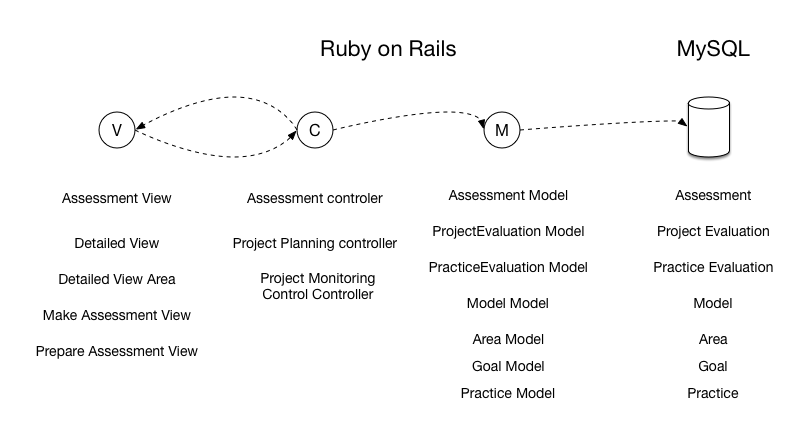
\includegraphics[scale=.3]{presentation.png}}
	\caption{Modelo de dados do SCRAIM}  
	\label{fig:figura}
\end{figure}

\subsection{Resultados}
Para determinar se a avaliação eletrónica gera resultados perto de uma avaliação manual realizada por um perito é necessário comparar uma avaliação automática (feita pela ferramenta) a uma avaliação manual (feita por um perito da área).

Nas duas avaliações apenas as duas áreas comtempladas na implementação atual são consideradas para esta comparação.

A distribuição da diferença e resultados que coincidem são mostrados na Figura
 \ref{fig:figura2}.

\begin{figure}[H]
	\centerline{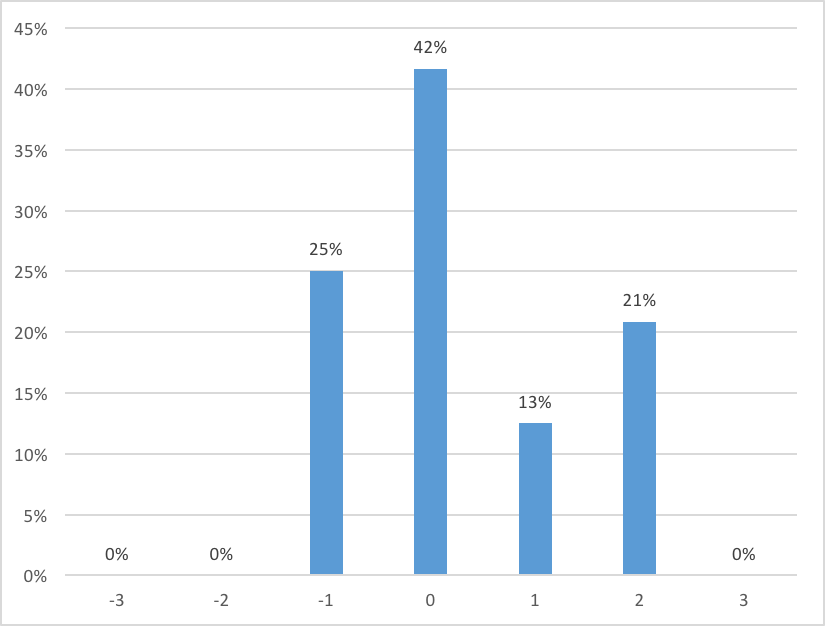
\includegraphics[scale=.5]{delta.png}}
	\caption{Distribuição dos erros eletrónicos}  
	\label{fig:figura2}
\end{figure}


É possível observar que nas avaliações eletrónicas automáticas que diferem 2 de uma avaliação manual são ainda 21\%.
A explicação para esta diferença é que atualmente é impossível verificar algum conteúdo de documentos submetidos no SCRAIM; em alguns casos apenas pelo uso do SCRAIM é automaticamente considerado o último nível ou algumas práticas são avaliadas em apenas dois níveis, o nível máximo (4) ou o nível mínimo (1). Por exemplo para a prática PP.SP1.1 é classificada de modo diferente, enquanto que na avaliação automática são apenas verificados os itens de trabalho, enquanto que na avaliação manual é verificado ainda os relatórios preliminares submetidos que contêm algumas evidencias para esta prática, sendo que não é possível verificar automaticamente ainda.

\subsection{Conclusões}

Todos os objetivos estabelecidos no inico desta dissertação foram quase todos completados e satisfeitos. O grupo de ferramentas, metodologias e técnicas atingidas resultaram num protótipo de avaliação automática como módulo do SCRAIM.
Os resultados gerados pelo protótipo são promissores, chegando muito perto dos valores de uma avaliação real. Era pretendido reduzir os custos e tempo de uma avaliação SCAMPI e com a análise comparativa feita podemos dizer que esta aproximação vai permitir isso e o protótipo depois de estendido e completado com o trabalho futuro vai facilitar as avaliações SCAMPI.



%%English version: comment first, uncomment second
\bibliographystyle{unsrt-pt}  % numeric, unsorted refs
%\bibliographystyle{unsrt}  % numeric, unsorted refs
\bibliography{refs}

\end{multicols}

\end{document}
